\documentclass[10pt, conference]{IEEEtran/IEEEtran}

\usepackage{graphicx}
\usepackage{color}
\usepackage{amsmath}
\usepackage{float}
\usepackage[all]{xy}
\usepackage[font=small]{caption}
\usepackage{hyperref}


\begin{document}

\title{Performance Analysis of TCP Variants}

\author{\IEEEauthorblockN{Liang Tian}
\IEEEauthorblockA{College of Computer and Information Science\\
Northeastern University, MA, 02115\\
Email: ltian@ccs.neu.edu\\}
\and
\IEEEauthorblockN{Yang Cai}
\IEEEauthorblockA{College of Computer and Information Science\\
Northeastern University, MA, 02115\\
Email: yang@ccs.neu.edu\\}
}
\maketitle
\begin{abstract}
In this paper we conduct simulation-based experiments to analyze performance of  TCP variants Tahoe, Reno, New Reno and Vegas, in particular their performances against congestion, as well as fairness between TCP variants for pairs Reno/Reno, New Reno/Reno, Vegas/Vegas, New Reno/Vegas. In addition, we analyze the influence of choice of queueing algorithms for Reno and SACK TCP.
\end{abstract}
\section{Introduction}
There are many TCP variants and many of them are implemented in some systems. In this paper we simulate Tahoe, Reno, New Reno and Vegas, compare their performances under congestion, as well as when they co-exit with other TCP variants (as in the real world). Also we explore the benefits of introducing SACK (selective acknowledgements)  and how well SACK works with RED and DropTail queueing disciplines.

As a quick review, we highlight some features we are interested in for each of the TCP variant \cite{sim}:

TCP Tahoe: \textit{Fast Retransmit}, after receiving a small number of duplicate acknowledgements for the same TCP segments (dup ACKs), the data sender infers that a packet has been lost and retransmits the packet without waiting for a retransmission timer to expire, leading to higher channel utilization and connection throughput.

TCP Reno: \textit{Fast Recovery}, prevents the communication path from going empty after Fast Retransmit, thereby avoiding the need to Slow-Start to re-fill it after a packet loss.

TCP New Reno: The New-Reno TCP in this paper includes a small change to the Reno algorithm at the sender that eliminates Reno's wait for a retransmit timer when multiple packets are lost from a window. \cite{sim}

Vegas TCP: TCP Vegas is a TCP congestion avoidance algorithm that emphasizes packet delay, rather than packet loss, as a signal to help determine the rate at which to send packets. TCP Vegas detects congestion at an incipient stage based on increasing Round-Trip Time (RTT) values of the packets in the connection unlike other flavors such as Reno, New Reno, etc., which detect congestion only after it has actually happened via packet loss. The algorithm depends heavily on accurate calculation of the Base RTT value. If it is too small then throughput of the connection will be less than the bandwidth available while if the value is too large then it will overrun the connection.
%
%A lot of research is going on regarding the fairness provided by the linear increase/decrease mechanism for congestion control in Vegas. 


\section{Methodology}

We use simulator \textit{ns2} which runs the experiment with given configuration specified in a tcl file, and
  output a trace file that we can analyze packets transmission. All computations and plots are done with Python.

We want to compare performances of TCP variants in the following scenarios: under congestion, co-existing with other variants under congestion, working with different queueing algorithms implemented at the gateways. The details specifications are given in each experiment in next section.
\subsection*{Notations}

We define throughput, latency, drop-rate as follows:

\[
\text{throughput}= \frac{\text{\# of received packets} \cdot \text{packet size}}{\text{duration of connection}}
\]
where we count the number of received unique ACKs at the sender agent and use it as \textbf{number of received packets}. Here ACKs must be unique because they could be duplicated, which means that there are packet losses.
\[
\text{latency}=\frac{\text{sum of RTT of all received packets} }{\text{\# of packets received}}
\]
where RTT is Round-Trip Time: we record the time it takes from a packet is enqueued at the sender agent(denoted as "+" in NS2 trace file) till the first ACK for the packet is received at the sender agent.
\[
\text{drop-rate}: \frac{\text{(\# sent packets - \# received packets)}}{\text{\# sent packets}}
\]
\section{Experiments}
In all experiments below, we use the same simple network topology as shown in the following graph:

\centerline{
\xymatrix{
N1 \ar@{-}[dr] & & & N4\\
& N2\ar@{-}[r]  & N3\ar@{-}[dr] \ar@{-}[ur]  & \\
N5\ar@{-}[ur]  &  &  & N6\\
}
}

\subsection{Experiment 1: TCP Performance Under Congestion}
\subsubsection{Configuration}

In this experiment, we want to explore performance of TCP variants under Congestion. So in each simulation, we set up a CBR source at N2 and sink at N3, between which there is a UDP data stream. One single TCP stream from N1 to N4 is introduced a few seconds after simulation starts.

To simulate different congestion levels, we vary CBR from 0.5 to 10 Mbps for each TCP variants Tahoe, Reno, New Reno and Vegas.


\subsubsection{Results Analysis}

\begin{figure}[!ht]
\begin{center}
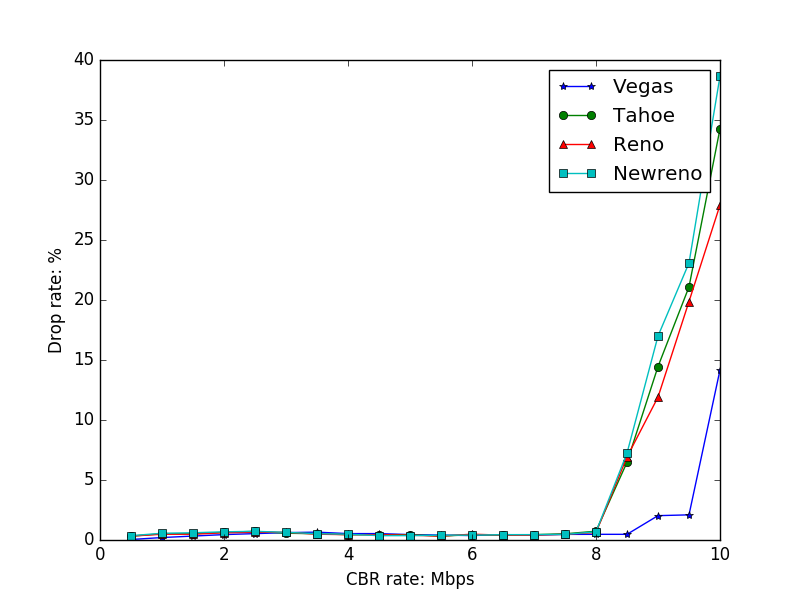
\includegraphics[width=\linewidth]{../exp1/exp1_drop.png}
\caption{Drop rate of TCP variants under different CBR rates}
\label{exp1_drop}
\end{center}
\end{figure}

\begin{figure}[!ht]
\begin{center}
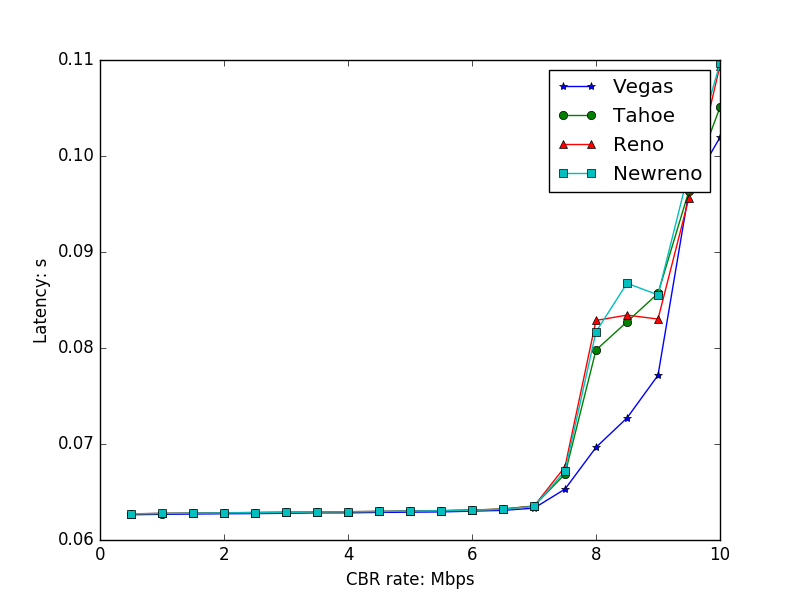
\includegraphics[width=\linewidth]{../exp1/exp1_lat.png}
\caption{Latency of TCP variants under different CBR rates}
\label{exp1_lat}
\end{center}
\end{figure}

\begin{figure}[!ht]
\begin{center}
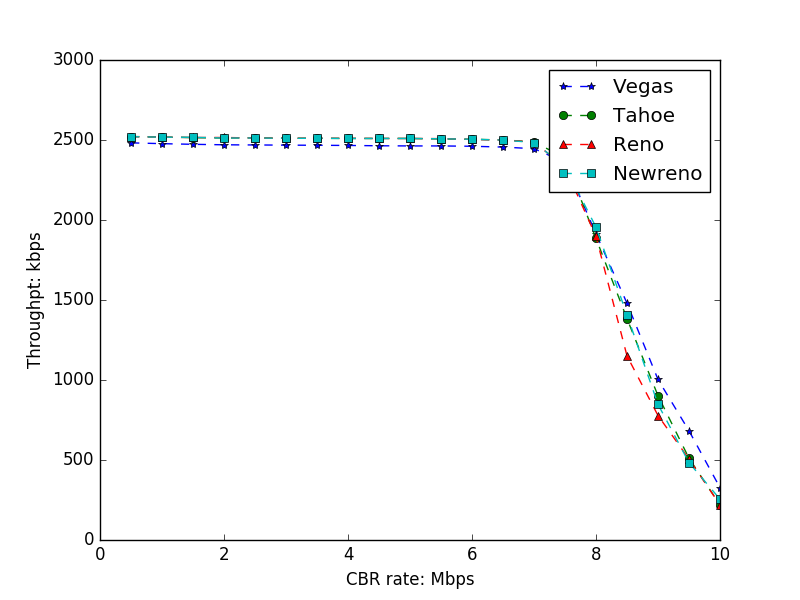
\includegraphics[width=\linewidth]{../exp1/exp1_thpt.png}
\caption{Throughput of TCP variants under different CBR rates}
\label{exp1_thpt}
\end{center}
\end{figure}

Fig. \ref{exp1_drop}, Fig. \ref{exp1_lat} and Fig. \ref{exp1_thpt} show the drop-rate, average latency and throughput for each TCP variant when the CBR rate varies from 0.5 to 10Mbps. 

We can see that when CBR rate is lower than 7Mbps, all TCP variants performs almost the same except Vegas has slightly lower throughput. When congestion becomes more and more severe, TCP Vegas starts to stand out while all others remain having similar performance. TCP Vegas has significantly lower drop-rate and level of latency and throughput is higher. So overall, TCP Vegas is better except that even when congestion level is low it already slows down slightly as it can detect congestion earlier than others\cite{vegas}.

To show that this is a statistically significant result, (i.e., it is the different implementations of TCP variants that is causing the difference in their average latency and drop-rate, instead of other parameters and random noise,) we run the simulation for each CBR rate for 10 times, each time we simulate with different values for the parameters

\begin{itemize}
\item start time of the TCP stream
\item packet size
\end{itemize}

\textbf{t-test}


\subsection{Experiment 2: Fairness Between TCP Variants}

In this experiment, we want to analyze fairness between TCP variants. To do so, we set up a CBR source at N2 and sink at N3 and a UDP stream between them. We start one TCP stream from N1 to N4 using one TCP
variant and another TCP stream from N5 to N6 using another TCP variant.

As in previous experiment, the configuration of the simulation iterate over the combinations of 
\begin{itemize}
\item Each pair of TCP variants(one of Reno/Reno, New Reno/Reno, Vegas/Vegas,
New Reno/Vegas), 
\item CBR from 0.5 to 10Mbps.
\end{itemize}

%Reno/Reno
\subsubsection{Reno/Reno}
\begin{figure}[!ht]
\begin{center}
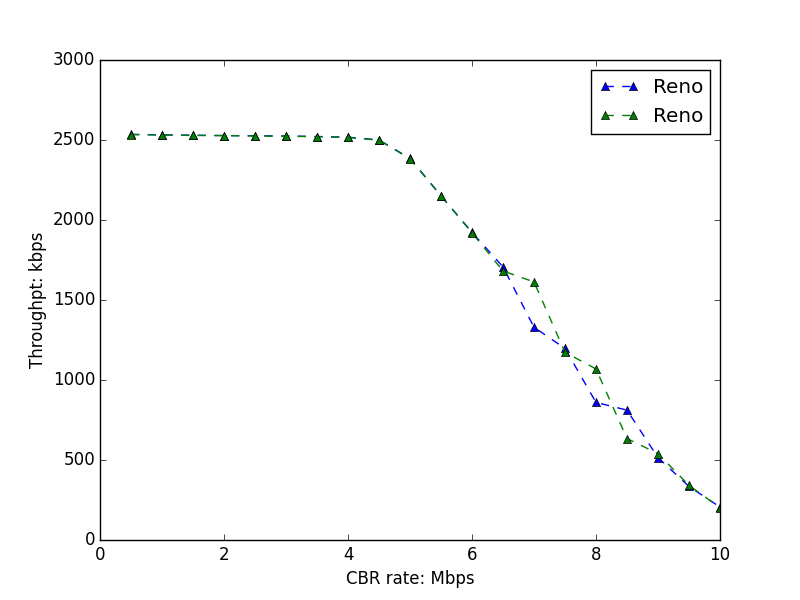
\includegraphics[width=\linewidth]{../exp2/exp2_Reno_Reno_thpt.png}
\caption{Throughput of Reno/Reno under different CBR rates}
\label{exp2_Reno_Reno_thpt}
\end{center}
\end{figure}

\begin{figure}[!ht]
\begin{center}
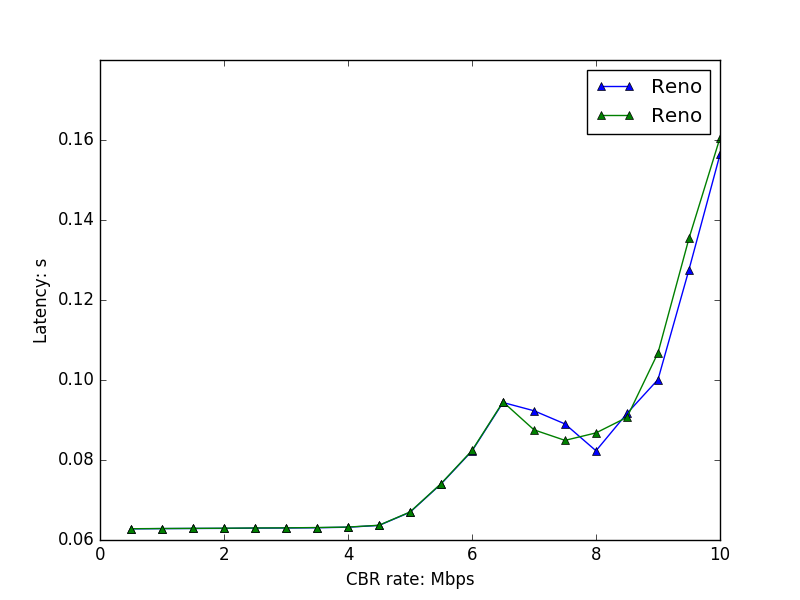
\includegraphics[width=\linewidth]{../exp2/exp2_Reno_Reno_lat.png}
\caption{Latency of Reno/Reno under different CBR rates}
\label{exp2_Reno_Reno_lat}
\end{center}
\end{figure}

\begin{figure}[!ht]
\begin{center}
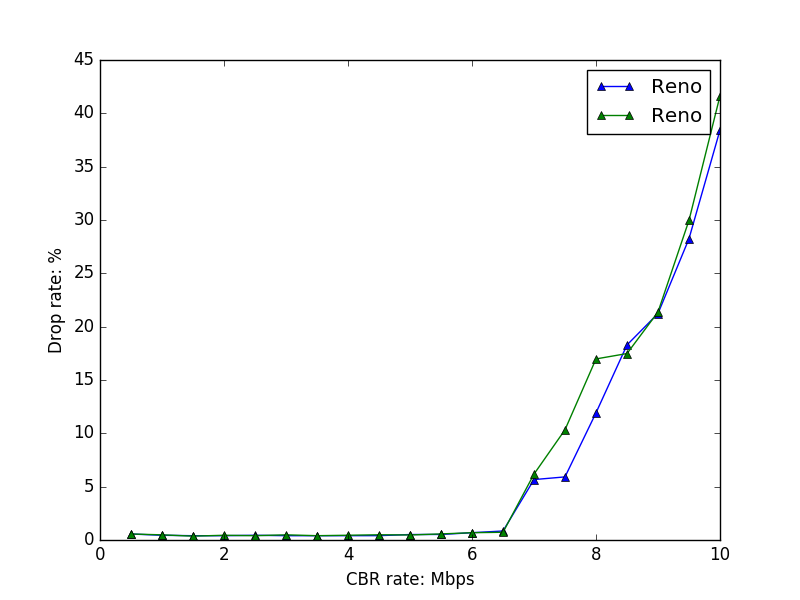
\includegraphics[width=\linewidth]{../exp2/exp2_Reno_Reno_drop.png}
\caption{Drop-rates of Reno/Reno under different CBR rates}
\label{exp2_Reno_Reno_drop}
\end{center}
\end{figure}


By comparing the drop-rate, throughput and latency of the two TCP streams in Fig. \ref{exp2_Reno_Reno_thpt}, \label{exp2_Reno_Reno_lat} and \label{exp2_Reno_Reno_drop}, we find that, very surprisingly, \textbf{Reno is not fair to itself}, when the available bandwidth is around the steam's normal throughput. We would have expected Reno is fair to itself as the two streams are using the same TCP variant with the same implementation. 

As have been discussed in \cite{reno}, ``TCP Reno induces packet losses to estimate the available bandwidth in the network. While there
are no packet losses, TCP Reno continues to increase its window size by one during each round
trip time. When it experiences a packet loss, it reduces its window size to one half of the current
window size. This is called additive increase and multiplicative decrease. Such
an algorithm leads to a fair allocation of bandwidth. TCP Reno, however, fails to achieve such
fairness because TCP is not a synchronized rate based control scheme, which is necessary for the
convergence.

The rate at which each connection updates its window size depends on the round trip delay of
the connection. Hence, the connections with shorter delays can update their window sizes faster
than other connections with longer delays, and thereby steal an unfair share of the bandwidth. As
a result, TCP Reno exhibits an undesirable bias against the connections with longer delays.'' Therefore, it's easy for one TCP Reno connection to become dominant over the other one, as shown in the figures.


%New Reno/Reno
\subsubsection{New Reno/Reno}
\begin{figure}[!ht]
\begin{center}
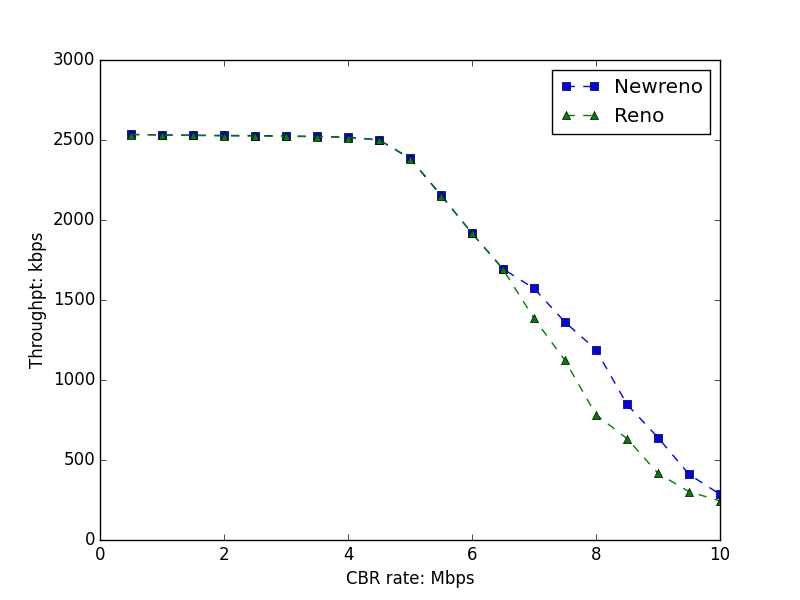
\includegraphics[width=\linewidth]{../exp2/exp2_Newreno_Reno_thpt.png}
\caption{Throughput of NewReno/Reno under different CBR rates}
\label{exp2_NewReno_Reno_thpt}
\end{center}
\end{figure}
\begin{figure}[!ht]
\begin{center}
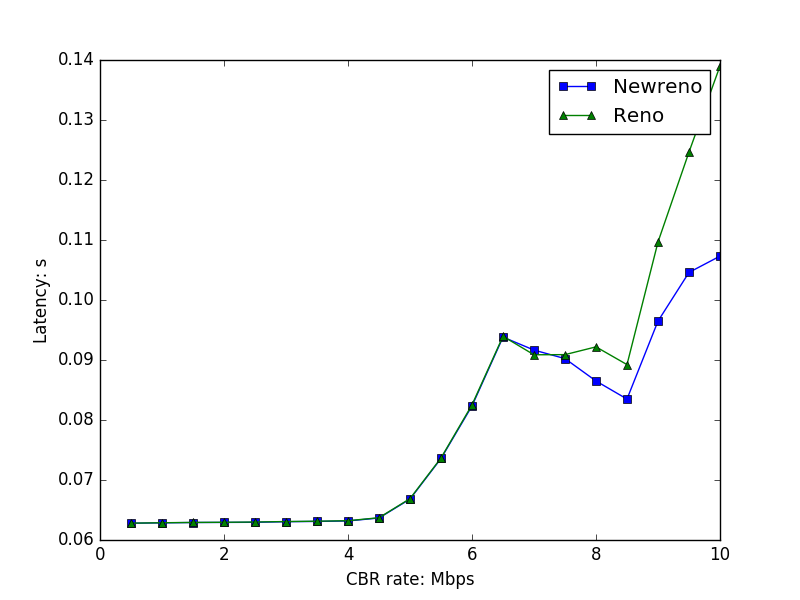
\includegraphics[width=\linewidth]{../exp2/exp2_Newreno_Reno_lat.png}
\caption{Latency of NewReno/Reno under different CBR rates}
\label{exp2_NewReno_Reno_lat}
\end{center}
\end{figure}
%Why?
Fig. \ref{exp2_NewReno_Reno_thpt} and Fig. \ref{exp2_NewReno_Reno_lat} shows throughput and latency of the two TCP NewReno streams. 

It's clear that New Reno is not fair to Reno. New Reno is getting more throughput and maintains lower latency when congestion level gets high. The reason for this is that, as stated in previous section and \cite{sim}, New Reno eliminates Reno's wait for a retransmit timer when multiple packets are lost from a window. So when multiple packets are lost, Reno will wait for a timeout before try to retransmit but New Reno will retransmit immediately, which helps New Reno to get lower latency and transmit more throughput.



\subsubsection{Vegas/Vegas}
% only 1 figure here.
\begin{figure}[!hb]
\begin{center}
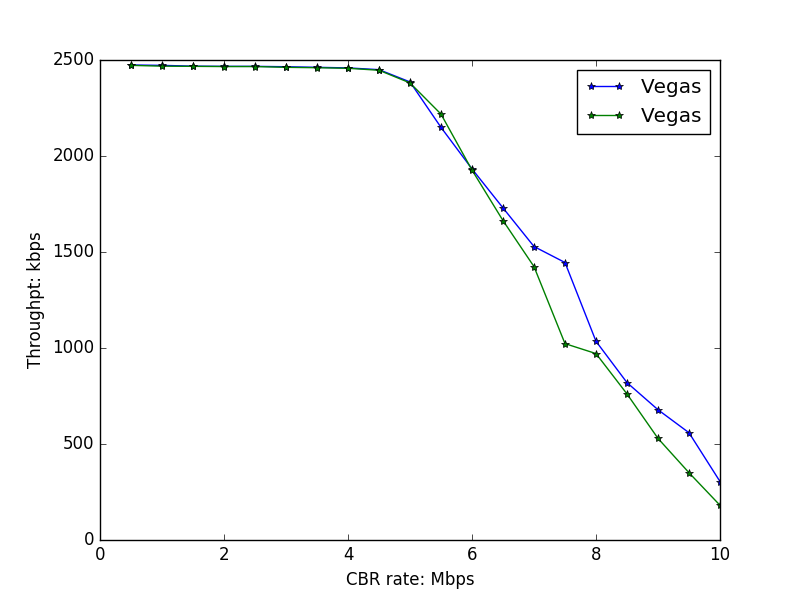
\includegraphics[width=\linewidth]{../exp2/exp2_Vegas_Vegas_thpt.png}
\caption{Throughput of Vegas/Vegas under different CBR rates}
\label{exp2_Vegas_Vegas_thpt}
\end{center}
\end{figure}
Vegas is fair to itself, as shown in Fig. \ref{exp2_Vegas_Vegas_thpt}. This is because unlike TCP Reno, Vegas'
window sizes converge to a point such that the queue sizes are within the same range for both connections, as shown in \cite{reno}.
%New Reno/Vegas
\subsubsection{New Reno/Vegas}


Performance of Vegas degrades because Vegas reduces its sending rate before New Reno, as it detects congestion early and hence gives greater bandwidth to co-existing TCP Reno flows. Also, New Reno inherits Reno's aggressive nature and is even more aggressive.
\begin{figure}[!h]
\begin{center}
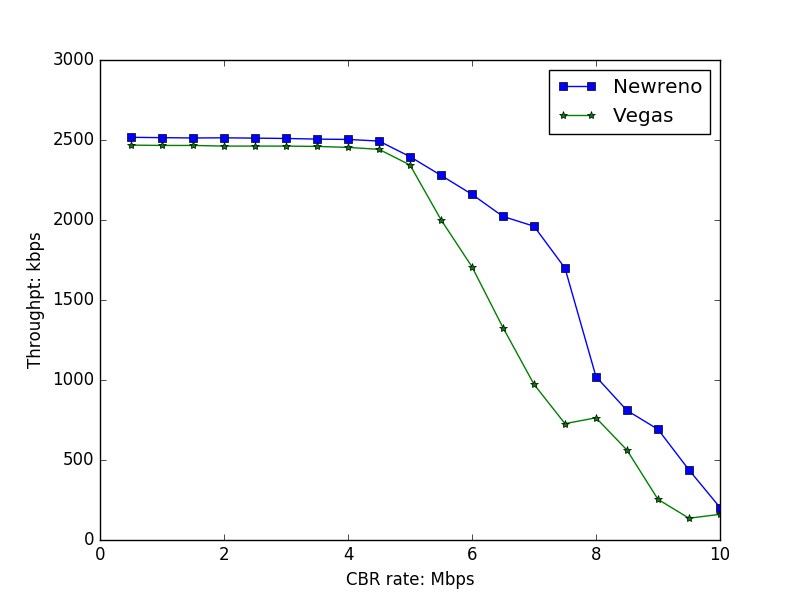
\includegraphics[width=\linewidth]{../exp2/exp2_Newreno_Vegas_thpt.png}
\caption{Throughput of New Reno/Vegas under different CBR rates}
\label{exp2_NewReno_Vegas_thpt}
\end{center}
\end{figure}




\subsection{Experiment 3: Influence of Queuing}

\subsubsection{Configuration}

For this experiment we want to study the influence of the queuing discipline used by nodes on the overall throughput of flows. We noticed with our choice of size of queue (10 in this experiment), the throughput of TCP connections is about 3Mbps. So we set the bandwidth available on the links to be 3Mbps, run a TCP stream from N1 to N4 and start a UDP stream at 3Mbps from N2 to N3 when TCP connection becomes stable (after about 10s to be safe) and see how RED and DropTail distribute bandwidth for 20 seconds.

\subsubsection{Results Analysis}

To compute how throughput, latency and drop-rate change over time, we split the duration into 30 segments, 1s each. For each segment we compute the stats separately and plot the graph using these 30 data points. On Fig. \ref{exp3_lat} and \ref{exp3_drop} there are many data points missing, which is because Reno and SACK cannot transmit any packet with DropTail, we can interpret those as 100\% drop-rate and infinite latency.

When CBR flow is introduced, TCP flows start dropping most packet and throughput drops to near 0.

It's not surprising to see that with RED, both SACK and Reno are getting some share of the bandwidth as RED is designed for congestion avoidance. They didn't get half the bandwidth mainly because TCP is slower compared to UDP by nature. But compare to DropTail, where SACK and Reno could barely send any packet, RED is fair.

\begin{figure}[!ht]
\begin{center}
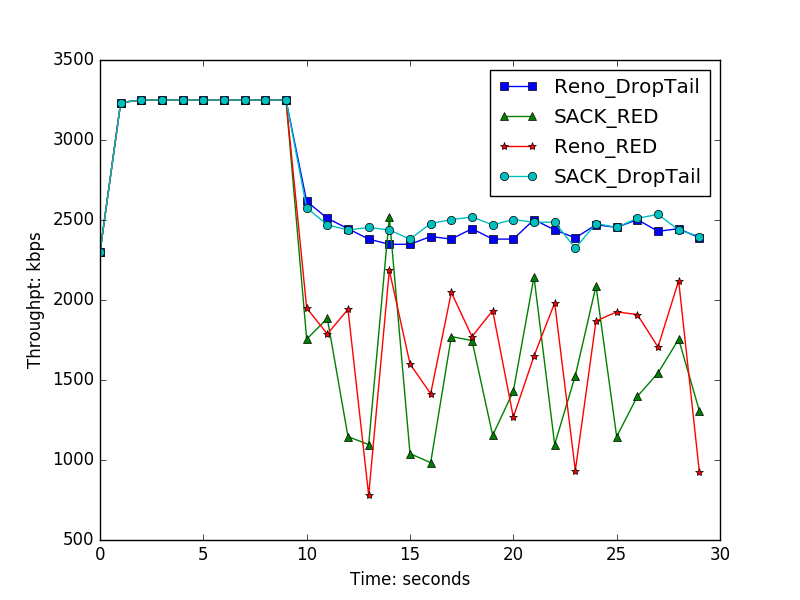
\includegraphics[width=\linewidth]{../exp3/exp3_thpt.png}
\caption{Throughput of TCP variants with different queueing algorithm}
\label{exp3_thpt}
\end{center}
\end{figure}

\begin{figure}[!ht]
\begin{center}
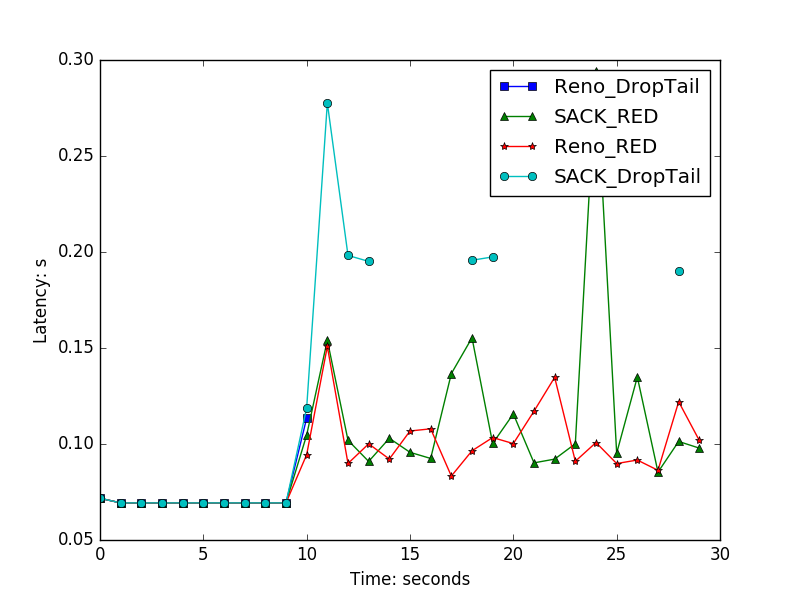
\includegraphics[width=\linewidth]{../exp3/exp3_lat.png}
\caption{Latency of TCP variants with different queueing algorithm}
\label{exp3_lat}
\end{center}
\end{figure}

\begin{figure}[!ht]
\begin{center}
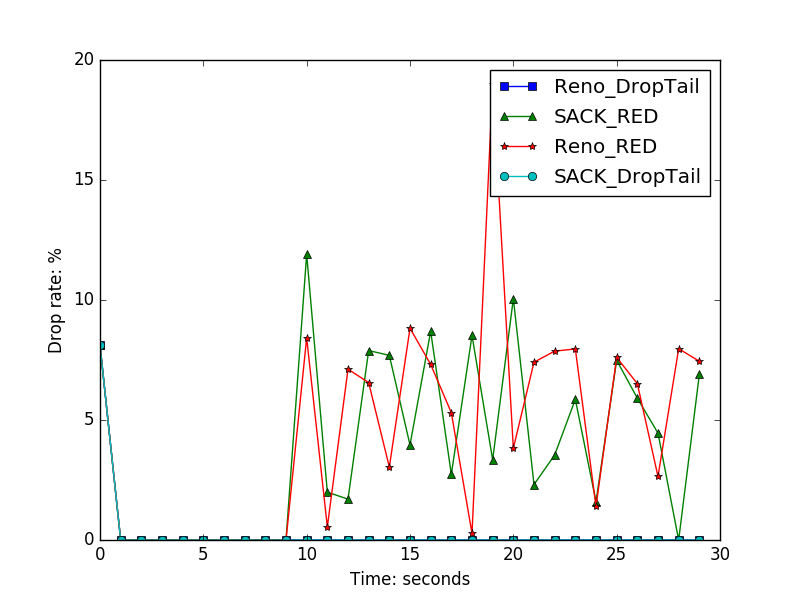
\includegraphics[width=\linewidth]{../exp3/exp3_drop.png}
\caption{Drop-rate of TCP variants with different queueing algorithm}
\label{exp3_drop}
\end{center}
\end{figure}


\section{Conclusion}
We explored the performance and fairness of TCP variants Tahoe, Reno, New Reno and Vegas, and influence of RED and DropTail algorithm on TCP Reno and SACK. TCP Vegas overall performs better than other variants and is fair to other connections, but variants like TCP Reno/TCP New Reno steal an unfair share of bandwidth from other connections (including TCP Vegas). RED is designed for congestion avoidance and does try to give each connection a fair share of bandwidth. As shown in \cite{reno}, RED gateways could be used to make TCP Vegas more compatible with TCP Reno in a competitive environment. In conclusion, we agree with \cite{vegas_red}, switching from Reno to Vegas will improve overall performance and these results lead us to believe that many would benefit from more widespread adoption of TCP Vegas and RED.

\begin{thebibliography}{50}
\bibitem{sim} Fall, Kevin, and Sally Floyd. ``Simulation-based comparisons of Tahoe, Reno and SACK TCP.''\textit{ACM SIGCOMM Computer Communication Review}
 26.3 (1996): 5-21.
 \bibitem{vegas}  \url{https://en.wikipedia.org/wiki/TCP_Vegas}
 \bibitem{vegas_red} Weigle, Eric, and Wu-chun Feng. ``A case for TCP Vegas in high-performance computational grids.'' 
 \textit{High Performance Distributed Computing, 2001. Proceedings. 10th IEEE International Symposium on}. IEEE, 2001. 
 \bibitem{reno} Mo, Jeonghoon, et al. ``Analysis and comparison of TCP Reno and Vegas.'' 
 \textit{IEEE INFOCOM. Vol. 3. INSTITUTE OF ELECTRICAL ENGINEERS INC} (IEEE), 1999.
 \bibitem{red} Floyd, Sally, and Van Jacobson. ``Random early detection gateways for congestion avoidance.'' \textit{IEEE/ACM Transactions on networking} 1.4 (1993): 397-413.
\end{thebibliography}



\end{document}
